\documentclass[journal]{IEEEtran}
% Format: IEEE journal (IEEEtran), as used by IEEE J-BHI.
% Every number in this paper comes from tables/numbers.tex and tables/*.tex, which are generated by
% scripts/make_tables.py from the result files in runs/freq_v1/results/ and claude_s/. Do not type numbers by hand.
% TODO: move the claude_s/ results (image weight, CheXpert labeler counts) into runs/freq_v1/results/.

\usepackage{amsmath,amssymb}
\usepackage{graphicx}
\usepackage{booktabs}
\usepackage{url}
\usepackage{cite}
\usepackage[hidelinks]{hyperref}
\newcommand{\NihROne}{+0.59}
\newcommand{\NihPOne}{0.025}
\newcommand{\NihRhoOne}{+0.50}
\newcommand{\NihPsOne}{0.069}
\newcommand{\NihSlopeOne}{+0.086}
\newcommand{\CxpROne}{+0.76}
\newcommand{\CxpPOne}{0.004}
\newcommand{\CxpRhoOne}{+0.83}
\newcommand{\CxpPsOne}{<0.001}
\newcommand{\CxpSlopeOne}{+0.304}
\newcommand{\NihWordROne}{+0.56}
\newcommand{\NihWordPOne}{0.036}
\newcommand{\NihRTwo}{-0.55}
\newcommand{\NihPTwo}{0.041}
\newcommand{\NihPartial}{-0.31}
\newcommand{\NihPartialP}{0.278}
\newcommand{\CxpRTwo}{-0.45}
\newcommand{\CxpPTwo}{0.143}
\newcommand{\CxpPartial}{+0.17}
\newcommand{\CxpPartialP}{0.608}
\newcommand{\NihWordRTwo}{-0.67}
\newcommand{\NihWordPTwo}{0.008}
\newcommand{\NihWordPartial}{-0.51}
\newcommand{\NihWordPartialP}{0.060}
\newcommand{\NihTrendZero}{+0.59}
\newcommand{\NihTrendRef}{+0.34}
\newcommand{\CxpTrendZero}{+0.76}
\newcommand{\CxpTrendRef}{+0.40}
\newcommand{\NihTrendAll}{+0.59, +0.60, +0.52, +0.53, +0.48, +0.46, +0.38, +0.34}
\newcommand{\NihImproved}{7}
\newcommand{\CxpImproved}{4}
\newcommand{\ZSMeanNih}{0.685}
\newcommand{\ZSMeanCxp}{0.757}
\newcommand{\NihZsGainR}{-0.59}
\newcommand{\NihZsGainP}{0.027}
\newcommand{\NihZsGainRho}{-0.38}
\newcommand{\NihZsGainPs}{0.185}
\newcommand{\CxpZsGainR}{-0.69}
\newcommand{\CxpZsGainP}{0.012}
\newcommand{\CxpZsGainRho}{-0.48}
\newcommand{\CxpZsGainPs}{0.118}
\newcommand{\PneuWord}{17.4}
\newcommand{\PneuAsserted}{5.7}
\newcommand{\AgreeCxpMin}{99.98}
\newcommand{\NihFcaRef}{0.703}
\newcommand{\NihGlobalRef}{0.710}
\newcommand{\NihRuleRef}{0.713}
\newcommand{\NihZsRef}{0.685}
\newcommand{\NihFcaBelow}{7}
\newcommand{\NihGlobalBelow}{5}
\newcommand{\NihRuleBelow}{5}
\newcommand{\CxpFcaRef}{0.769}
\newcommand{\CxpGlobalRef}{0.810}
\newcommand{\CxpRuleRef}{0.814}
\newcommand{\CxpZsRef}{0.757}
\newcommand{\CxpFcaBelow}{8}
\newcommand{\CxpGlobalBelow}{5}
\newcommand{\CxpRuleBelow}{5}
\newcommand{\AlphaGlobalRef}{0.020}
\newcommand{\RuleB}{-0.3}
\newcommand{\RuleBNeg}{6}
\newcommand{\NK}{7}
\newcommand{\AlphaRuleMin}{0.008}
\newcommand{\AlphaRuleMax}{0.032}
\newcommand{\NihGlobalVsFca}{+0.0073 [+0.0042, +0.0103]}
\newcommand{\NihRuleVsGlobal}{+0.0026 [+0.0023, +0.0030]}
\newcommand{\NihFcaSigBetter}{7}
\newcommand{\NihFcaSigWorse}{6}
\newcommand{\NihGlobalSigBetter}{8}
\newcommand{\NihGlobalSigWorse}{5}
\newcommand{\NihRuleSigBetter}{8}
\newcommand{\NihRuleSigWorse}{4}
\newcommand{\NihNBoot}{200}
\newcommand{\CxpGlobalVsFca}{+0.0412 [+0.0178, +0.0653]}
\newcommand{\CxpRuleVsGlobal}{+0.0038 [+0.0014, +0.0064]}
\newcommand{\CxpFcaSigBetter}{1}
\newcommand{\CxpFcaSigWorse}{4}
\newcommand{\CxpGlobalSigBetter}{1}
\newcommand{\CxpGlobalSigWorse}{3}
\newcommand{\CxpRuleSigBetter}{1}
\newcommand{\CxpRuleSigWorse}{1}
\newcommand{\CxpNBoot}{1000}
\newcommand{\MimicCxrPatients}{65{,}379}
\newcommand{\NTest}{25{,}596}
\newcommand{\NTestPatients}{2{,}797}
\newcommand{\NCxpVal}{200}
\newcommand{\NCxpTest}{500}
\newcommand{\NCxpSupp}{10{,}000}
\newcommand{\MimicCxrPairs}{377{,}110}
\newcommand{\MimicCxrStudies}{227{,}835}
\newcommand{\MimicCxrUniqueTexts}{133{,}737}
\newcommand{\MimicCxrNoImpression}{57{,}000}
\newcommand{\NCkpt}{236}
\newcommand{\BestStep}{46{,}400}
\newcommand{\BestEpoch}{7.87}
\newcommand{\SelAUC}{0.713}
\newcommand{\CxpBestStep}{32{,}200}
\newcommand{\CxpBestEpoch}{5.46}
\newcommand{\CxpSelAUC}{0.858}
\newcommand{\KRef}{64}


\begin{document}

\title{Pretraining Report Frequency, Zero-Shot Performance and Few-Shot Adaptation of a Chest X-Ray
Vision--Language Model: A Preliminary Study}

\author{First~Author, Second~Author, and Third~Author
\thanks{PRELIMINARY DRAFT, not for distribution. Results are from a single model.}}

\maketitle

\begin{abstract}

Few-shot adaptation of medical vision--language models has been motivated by the claim that zero-shot performance is limited for concepts that are rare in the pretraining data. 
We measured concept frequency as asserted, not merely mentioned, findings in the \MimicCxrPairs{} MIMIC-CXR image--text pairs that trained CheXzero, related it to zero-shot performance and few-shot gain, and used it to set a per-class weight in few-shot adaptation.
Concept frequency was measured as the share of impressions in which the CheXpert labeler, extended to the 14 ChestX-ray14 classes, marks a finding as present. 
Denied findings were not counted.
As reported for general-domain models, zero-shot area under the ROC curve (AUC) increased with log concept frequency, on ChestX-ray14 (r = \NihROne, p = \NihPOne) and on CheXpert (r = \CxpROne, p = \CxpPOne).
With \KRef{} support images per class, rarely asserted ChestX-ray14 classes gained more from few-shot adaptation (r = \NihRTwo, p = \NihPTwo), but the association was not significant after controlling for zero-shot AUC (partial r = \NihPartial, p = \NihPartialP).
A low zero-shot AUC was itself associated with a larger gain.
A smaller global image weight, tuned on ChestX-ray14 and applied to CheXpert without retuning, raised the mean AUC from \NihFcaRef{} to \NihGlobalRef{} and from \CxpFcaRef{} to \CxpGlobalRef{}.
Setting the weight per class from concept frequency raised it further, to \NihRuleRef{} and \CxpRuleRef{}.
Pretraining concept frequency thus provides a per-class image weight for few-shot adaptation that transfers across datasets without retuning.


% Rarely asserted classes gained more from few-shot adaptation (SS-Text, $K=\KRef$; ChestX-ray14 $r=\NihRTwo$, $p=\NihPTwo$), but after controlling for zero-shot AUC the association was not significant (partial $r=\NihPartial$, $p=\NihPartialP$), whereas a low zero-shot AUC was itself associated with a larger gain. 
% With its published weighting, SS-Text made \NihFcaBelow{} of 14 ChestX-ray14 classes and \CxpFcaBelow{} of 12 CheXpert classes worse than zero-shot, mostly frequently asserted ones. 
% A smaller weight on the support images, chosen on ChestX-ray14 and applied to CheXpert unchanged, reduced this harm (mean AUC at $K=\KRef$: \NihFcaRef{} $\rightarrow$ \NihGlobalRef{} and \CxpFcaRef{} $\rightarrow$ \CxpGlobalRef{}), and setting the weight per class from $f$ added a small further gain (\NihRuleRef{} and \CxpRuleRef{}).
\end{abstract}

\begin{IEEEkeywords}
Chest X-ray, vision--language models, zero-shot classification, few-shot adaptation, concept frequency.
\end{IEEEkeywords}

% =================================================================================================
\section{Introduction}

Contrastive vision--language pretraining (CLIP~\cite{radford2021clip}) learns a joint embedding of
images and text, so a classifier for any class can be built from a text prompt alone. CheXzero
applied this to chest radiographs, training on MIMIC-CXR images paired with the impression sections
of their radiology reports, and reached radiologist-level performance on several findings without
labelled training images~\cite{tiu2022chexzero}.

Such models are not ``zero-shot'' in the strict sense: the class names appear in the pretraining
text. In general-domain models, Udandarao \emph{et al.}~\cite{udandarao2024zeroshot} found
\emph{``a consistent linear relationship between CLIP's zero-shot performance on a concept and the
log-scaled pretraining concept frequency.''} Parashar \emph{et al.}~\cite{parashar2024neglected} estimated
concept frequency from pretraining captions and used it to improve rare concepts: they prompt with the
most frequent synonym of a class name and train a linear classifier on a small, balanced set of retrieved
pretraining data.

This finding is also used to motivate few-shot adaptation. The Full Conformal Adaptation paper, whose
training-free solver SS-Text we use, states that zero-shot \emph{``performance vanishes when specific
domains and concepts are represented with low frequency during pre-training''} and that zero-shot
performance \emph{``is limited to the pre-training concept frequency and therefore requires
adaptation''}~\cite{silvarodriguez2025fca}. That work cites~\cite{udandarao2024zeroshot} for this
claim but does not measure concept frequency in its own models. Radiology also differs from web captions in a way that matters for the
measurement: reports routinely \emph{deny} findings (``no pneumothorax''), so a word count need not
reflect how often a finding was actually reported.

We test this motivation class by class, in one model and on two test sets:
\begin{enumerate}
\item \textbf{Relationship (1):} does zero-shot AUC increase with the log-frequency $f$ of the finding?
\item \textbf{Relationship (2):} does the few-shot gain $\Delta$AUC \emph{decrease} with $\log f$, and
does $f$ predict it beyond the zero-shot AUC?
\end{enumerate}
Writing them as straight lines over $\log_{10} f$,
\begin{equation}
\mathrm{AUC}_{\mathrm{zs}} = a\log_{10} f + b, \qquad \Delta\mathrm{AUC}_{\mathrm{fs}} = c\log_{10} f + d,
\end{equation}
the hypothesis is $a>0$ and $c<0$. The first equation is our formalization of the log-linear trend
described in~\cite{udandarao2024zeroshot}.

Our findings are: (i) relationship (1) holds on both test sets with a negation-aware frequency;
(ii) relationship (2) points the expected way but is not significant once the zero-shot AUC is
controlled for; and (iii) with its published weighting, SS-Text lowers the AUC of many classes, mostly
frequently asserted ones; a smaller weight on the support images reduces this harm, and a weight set per
class from $f$ adds a small further gain.



% =================================================================================================
\section{Related Work}

\emph{Pretraining frequency and zero-shot performance.} Udandarao \emph{et
al.}~\cite{udandarao2024zeroshot} counted concepts in the pretraining data of general-domain CLIP models
and found zero-shot performance to grow log-linearly with concept frequency. Parashar \emph{et
al.}~\cite{parashar2024neglected} estimated frequency from pretraining captions and used it to improve
rare concepts through the choice of prompt and retrieved pretraining data. Both studies use web
image--caption data, where captions rarely deny what is absent; we measure frequency in radiology
reports with a negation-aware labeler, and on a medical model.

\emph{Few-shot adaptation without training.} Training-free adapters combine the text classifier of a
vision--language model with features of a few labelled images. Tip-Adapter~\cite{zhang2022tip}
blends a cache of support features with the zero-shot classifier through one global weight. SS-Text, the
solver of Full Conformal Adaptation~\cite{silvarodriguez2025fca}, adds the summed support features to
the text prototypes, with a weight that shrinks the role of the text as the support set grows; its
authors evaluate it on medical models, including a chest X-ray model, and report results averaged over
classes. We use SS-Text and examine its effect class by class, together with the image weight.

% =================================================================================================
\section{Materials and Methods}

\subsection{Data}
Table~\ref{tab:data} summarizes the datasets and splits.

\emph{Training:} MIMIC-CXR-JPG~\cite{johnson2019mimiccxrjpg}, \MimicCxrPairs{} images from \MimicCxrStudies{} studies
of \MimicCxrPatients{} patients. Following CheXzero~\cite{tiu2022chexzero}, the text paired with each image
is the impression section of its report; reports without an impression section become the literal text
``NO IMPRESSION'' (\MimicCxrNoImpression{} rows). A study's impression is paired with each of its images, so the
training set has \MimicCxrPairs{} image--text pairs but only \MimicCxrUniqueTexts{} distinct texts. No labels are used
for training.

\emph{ChestX-ray14:} the official test split~\cite{wang2017chestxray8} (\NTest{} images from
\NTestPatients{} patients; 14 findings, labels mined from the reports). A pool of 20{,}000 images drawn
from the official train/validation split, which shares no patient with the test split, is divided by a
fixed random permutation into a \emph{selection set} (6{,}000 images, used to choose the checkpoint and
the few-shot image weight) and a \emph{support set} (14{,}000 images, the source of few-shot examples).

\emph{CheXpert:} the 500-study test set and the 200-study validation set, one frontal image per study,
with the 12 pathology labels (No Finding and Support Devices excluded); the validation set is used only
to choose the checkpoint, with CheXzero's 5 labels. Few-shot examples come from a fixed random subset of
\NCxpSupp{} frontal training images; a blank training label counts as negative and an uncertain one
($-1$) is never drawn.

\begin{table*}[!t]
\centering
\footnotesize
\caption{Datasets and splits. MIMIC-CXR provides image--text pairs (one row per image; a study's impression is
repeated for each of its images); no labels are used for training. ChestX-ray14 selection and support are drawn from
the official train/validation split and test is the official test split. CheXpert: one frontal image per study for
validation and test; the support images are a fixed random subset of the training set. Last column: images
positive for at least one of the labels used in that set.}
\label{tab:data}
\begin{tabular}{llrrlr}
\toprule
Set & Role & Images & Patients & Labels used & $\geq$1 positive (\%) \\
\midrule
MIMIC-CXR & training & 377{,}110 & 65{,}379 & impression text & -- \\
ChestX-ray14 selection & checkpoint choice & 6{,}000 & 4{,}062 & 14 labels & 39.2 \\
ChestX-ray14 support & few-shot examples & 14{,}000 & 7{,}646 & 14 labels & 39.4 \\
ChestX-ray14 test & evaluation & 25{,}596 & 2{,}797 & 14 labels & 61.5 \\
CheXpert validation & checkpoint choice & 200 & 200 & 5 labels & 64.0 \\
CheXpert train subset & few-shot examples & 10{,}000 & 8{,}429 & 12 labels & 84.3 \\
CheXpert test & evaluation & 500 & 500 & 12 labels & 70.4 \\
\bottomrule
\end{tabular}
\end{table*}


\subsection{Model and training}
We followed the CheXzero recipe~\cite{tiu2022chexzero}: a CLIP ViT-B/32 image encoder and text
transformer initialized from CLIP weights, trained contrastively for 8 epochs (SGD, learning rate
$10^{-4}$, momentum 0.9, batch size 64), saving a checkpoint every 200 steps (\NCkpt{} checkpoints).
We use a single checkpoint per test set (no ensemble).

\subsection{Concept frequency}
For each class, $f$ is the percentage of the \MimicCxrPairs{} training pairs whose impression asserts the finding.
We ran the CheXpert labeler~\cite{irvin2019chexpert} on every training impression. 
The labeler finds mentions of a finding with lists of phrases, classifies each mention as negated, uncertain or positive with rules on the sentence's dependency parse, which build on NegBio~\cite{peng2018negbio}, and combines the mentions into one label per report: positive if any mention is positive, otherwise uncertain if any is uncertain, otherwise negative.
A pair counts if its report is labelled positive; pairs whose training text is ``NO IMPRESSION'' are never counted.
Uncertain mentions (``possible effusion'') are not counted.

The labeler covers 7 of the 14 ChestX-ray14 classes. For the other 7 we added one mention-phrase file
each (Emphysema: \emph{emphysema}; Fibrosis: \emph{fibrosis}; Hernia: \emph{hernia}; Infiltration:
\emph{infiltrat}; Mass: \emph{mass}, \emph{masses}; Nodule: \emph{nodule}, \emph{nodulation}; Pleural
Thickening: \emph{pleural thicken}; the Infiltration and Pleural Thickening entries match any word
starting with these letters) and left the negation and uncertainty rules and all code unchanged.
For the classes the labeler already covers, its output agreed with the labels released with
MIMIC-CXR-JPG~\cite{johnson2019mimiccxrjpg} on at least \AgreeCxpMin\% of the training pairs that have an
impression, for every class.

For comparison on ChestX-ray14 we also use two \emph{word} counts, which include denials: a pair counts
if its impression contains the class name as consecutive word stems (Snowball English
stemmer~\cite{porter2001snowball}, which joins forms such as \emph{infiltration/infiltrate}), or, in the
second count, as the exact name.

\subsection{Zero-shot classification and checkpoint selection}
Each class is scored with CheXzero's prompt pair, ``\{label\}'' versus ``no \{label\}''. Let
$v=g(x)\in\mathbb{R}^{512}$ be the embedding of a test image $x$ produced by the image encoder $g$, and
$t_{\mathrm{pos}}=h(\text{``\{label\}''})$, $t_{\mathrm{neg}}=h(\text{``no \{label\}''})$ the embeddings of
the two prompts produced by the text encoder $h$; all embeddings are normalized to unit length, so a dot
product is a cosine similarity. The score of image $x$ for the class is
\begin{equation}
p(x)=\sigma\!\left(v\cdot t_{\mathrm{pos}} - v\cdot t_{\mathrm{neg}}\right)
=\frac{e^{\,v\cdot t_{\mathrm{pos}}}}{e^{\,v\cdot t_{\mathrm{pos}}}+e^{\,v\cdot t_{\mathrm{neg}}}},
\label{eq:zs}
\end{equation}
where $\sigma$ is the logistic sigmoid; the right-hand form shows that it is a two-way softmax over the
prompts. Since AUC depends only on the ranking of $p$ across images, no temperature is applied.
Two ChestX-ray14 class names are rephrased for the prompt (``Effusion'' $\rightarrow$ ``Pleural
Effusion''; ``Pleural\_Thickening'' $\rightarrow$ ``Pleural Thickening''). All \NCkpt{} checkpoints were
scored and, for each test set, the one with the highest mean AUC was kept: on the ChestX-ray14
selection set (step \BestStep, epoch \BestEpoch; AUC \SelAUC) and on the CheXpert validation set (step
\CxpBestStep, epoch \CxpBestEpoch; AUC \CxpSelAUC).

\subsection{Few-shot adaptation}
We use SS-Text, the training-free solver of~\cite{silvarodriguez2025fca} (Eq.~10). The encoders $g$ and
$h$ stay frozen and no layer is added or trained; adaptation only changes the two vectors that a test
image is compared with in~\eqref{eq:zs}.

For one class and a given $K$, let $\mathcal{P}_K$ be $K$ images drawn at random from the support set
among those labelled positive for the class, and $\mathcal{N}_K$ be $K$ images drawn among those
labelled negative for it, with embeddings $v_i=g(x_i)$. The text prototypes are replaced by
\begin{equation}
w_{\mathrm{pos}} = t_{\mathrm{pos}} + \alpha\!\sum_{i\in\mathcal{P}_K} v_i, \qquad
w_{\mathrm{neg}} = t_{\mathrm{neg}} + \alpha\!\sum_{i\in\mathcal{N}_K} v_i,
\label{eq:sstext}
\end{equation}
and every test image is scored with~\eqref{eq:zs} using $w_{\mathrm{pos}}, w_{\mathrm{neg}}$ in place of
$t_{\mathrm{pos}}, t_{\mathrm{neg}}$:
\begin{equation}
p_K(x)=\sigma\!\left(v\cdot w_{\mathrm{pos}} - v\cdot w_{\mathrm{neg}}\right).
\end{equation}
In words, ``what the class looks like'' becomes the prompt \emph{plus} a weighted sum of $K$ real
examples of it, and likewise for its absence. The score is linear in $v$, so
$w_{\mathrm{pos}}-w_{\mathrm{neg}}$ plays the role of the weight vector of a linear classifier, obtained by
one addition rather than by gradient descent. Each class gets its own pair $(w_{\mathrm{pos}}, w_{\mathrm{neg}})$.

The \emph{image weight} $\alpha$ sets how much the support images count relative to the prompt. In Eq.~10
of~\cite{silvarodriguez2025fca} the images are weighted by $1/(\lambda N\tau)$, and the authors fix
$\lambda=1/(N\tau)$, which gives $\alpha=1$, motivated by \emph{``diminishing the effect of textual priors as
more support data is available''}. With $\alpha=1$ and $K$ unit-length image vectors, the text vector
contributes roughly $1/(K+1)$ of each prototype. We compare three choices:
\begin{itemize}
\item \textbf{SS-Text:} $\alpha=1$, as published.
\item \textbf{Global $\alpha$:} one $\alpha$ for all classes, chosen for each $K$ on the ChestX-ray14
selection set from a grid of $\log_{10}\alpha$ between $-3$ and $1$ in steps of 0.1.
\item \textbf{Frequency rule:} a per-class weight
$\log_{10}\alpha_c = a + b\,(\log_{10} f_c - \overline{\log_{10} f})$, where the mean is over the classes of the
test set. The two numbers $a$ and $b$ are chosen for each $K$ on the ChestX-ray14 selection set, by grid search
($a$ as above, $b$ between $-1.5$ and $1$ in steps of 0.1; $b=0$ recovers the global $\alpha$); $b<0$ gives frequently asserted classes a smaller image weight.
\end{itemize}

A single weight shared by all classes follows Tip-Adapter \cite{zhang2022tip}, whose residual ratio $\alpha$ balances the few-shot image term against CLIP's text classifier; its authors set $\alpha$ larger when the domain gap to the pretraining data is larger, but use one value for all classes of a dataset. (?? check it again.)

Both are chosen to maximize the mean AUC over classes on the selection set, averaged over the support
draws. The choices are made once on ChestX-ray14 and applied to CheXpert without retuning. Choosing them uses
the labels of the selection set; after that, the frequency rule needs only $f$, which comes from the
pretraining text.

We use $K\in\{1,2,4,8,16,32,64\}$, each repeated with 20 independent draws of $\mathcal{P}_K$ and
$\mathcal{N}_K$; the draws are the same for all three choices. For each class and $K$ we report the AUC
averaged over the draws. $K$ is capped by the number of available positives. The few-shot gain of a
class is $\Delta\mathrm{AUC}=\mathrm{AUC}_K-\mathrm{AUC}_{\mathrm{zs}}$; unless stated otherwise it refers
to SS-Text.

\subsection{Statistics}
Each class is one point ($n=14$ for ChestX-ray14, $n=12$ for CheXpert). We fit ordinary least squares on
$\log_{10} f$ and report Pearson's $r$ and Spearman's $\rho$ with two-sided $p$-values. To separate the
effect of frequency on the few-shot gain from that of the starting AUC, we report the partial correlation
of $\Delta$AUC with $\log_{10} f$ after removing a linear effect of the zero-shot AUC from both. To compare
image weights at $K=\KRef$ we resample the test images with replacement (\NihNBoot{} resamples for
ChestX-ray14, \CxpNBoot{} for CheXpert), recompute every class's AUC on each resample with the support
draws fixed, and report 95\% percentile intervals of the paired differences, both for the mean over
classes and for each class's gain over zero-shot. A class is called significantly better or worse than
zero-shot when its interval excludes 0.

% =================================================================================================
\section{Results}

\begin{table}[!t]
\centering
\footnotesize
\caption{ChestX-ray14 classes: concept frequency $f$ in the MIMIC-CXR training impressions (\% of 377{,}110
image--text pairs; asserted = labelled positive by the CheXpert labeler; word = class name, stemmed or exact),
zero-shot AUC on the test set, and few-shot (SS-Text) gain at $K=64$ (mean of 20 draws).}
\label{tab:classes}
\setlength{\tabcolsep}{3pt}
\begin{tabular}{lrrrrrr}
\toprule
Class & \multicolumn{3}{c}{$f$ (\%)} & Test & Zero-shot & $\Delta$AUC \\
 & assert. & word & exact & pos. & AUC & $K{=}64$ \\
\midrule
Effusion & 15.59 & 24.17 & 15.55 & 4,658 & 0.769 & -0.014 \\
Atelectasis & 12.75 & 15.19 & 15.19 & 3,279 & 0.670 & -0.026 \\
Cardiomegaly & 12.05 & 7.67 & 7.67 & 1,069 & 0.833 & +0.027 \\
Edema & 7.89 & 14.37 & 14.37 & 925 & 0.802 & -0.031 \\
Pneumonia & 5.72 & 17.42 & 17.42 & 555 & 0.679 & -0.045 \\
Consolidation & 3.09 & 7.37 & 6.50 & 1,815 & 0.699 & +0.012 \\
Pneumothorax & 2.80 & 12.18 & 12.18 & 2,665 & 0.720 & -0.008 \\
Emphysema & 1.24 & 1.33 & 1.33 & 1,093 & 0.544 & +0.107 \\
Nodule & 0.98 & 1.42 & 0.74 & 1,623 & 0.532 & +0.059 \\
Mass & 0.79 & 1.17 & 1.01 & 1,748 & 0.694 & -0.038 \\
Hernia & 0.70 & 0.77 & 0.77 & 86 & 0.735 & +0.060 \\
Infiltration & 0.44 & 0.98 & 0.09 & 6,112 & 0.685 & -0.010 \\
Pleural Thickening & 0.41 & 0.64 & 0.64 & 1,143 & 0.660 & +0.033 \\
Fibrosis & 0.23 & 0.31 & 0.31 & 435 & 0.574 & +0.115 \\
\midrule
Mean & & & & & 0.685 & +0.017 \\
\bottomrule
\end{tabular}
\end{table}

\begin{table}[!t]
\centering
\footnotesize
\caption{CheXpert classes: asserted frequency $f$ in the training impressions, positives in the 500-study
test set, zero-shot AUC and few-shot (SS-Text) gain at $K=64$ (mean of 20 draws).}
\label{tab:cxpclasses}
\setlength{\tabcolsep}{3pt}
\begin{tabular}{lrrrr}
\toprule
Class & $f$ & Test & Zero-shot & $\Delta$AUC \\
 & (\%) & pos. & AUC & $K{=}64$ \\
\midrule
Pleural Effusion & 15.59 & 104 & 0.923 & -0.013 \\
Lung Opacity & 15.33 & 264 & 0.908 & -0.003 \\
Atelectasis & 12.75 & 153 & 0.837 & -0.072 \\
Cardiomegaly & 12.05 & 151 & 0.899 & -0.063 \\
Edema & 7.89 & 78 & 0.882 & -0.047 \\
Pneumonia & 5.72 & 11 & 0.759 & -0.082 \\
Consolidation & 3.09 & 29 & 0.885 & -0.006 \\
Pneumothorax & 2.80 & 9 & 0.679 & +0.082 \\
Lung Lesion & 2.34 & 8 & 0.554 & +0.159 \\
Enlarged Cardiomediastinum & 1.86 & 253 & 0.839 & -0.365 \\
Fracture & 1.55 & 5 & 0.377 & +0.191 \\
Pleural Other & 0.68 & 4 & 0.540 & +0.364 \\
\midrule
Mean & & & 0.757 & +0.012 \\
\bottomrule
\end{tabular}
\end{table}


\subsection{Concept frequency}
Asserted frequency spans more than an order of magnitude on both test sets (Tables~\ref{tab:classes}
and~\ref{tab:cxpclasses}). It can differ greatly from the word count: Pneumonia, for example, is named
in \PneuWord\% of training pairs but asserted in only \PneuAsserted\%, because the labeler does not
count denied or uncertain mentions.

\subsection{Relationship (1): zero-shot AUC}
Zero-shot AUC averaged \ZSMeanNih{} on ChestX-ray14 and \ZSMeanCxp{} on CheXpert. It increased with
log-frequency on both test sets (Table~\ref{tab:rel}, Fig.~\ref{fig:rel}): \NihSlopeOne{} AUC per decade
on ChestX-ray14 ($r=\NihROne$, $p=\NihPOne$; $\rho=\NihRhoOne$, $p=\NihPsOne$) and \CxpSlopeOne{} on
CheXpert ($r=\CxpROne$, $p=\CxpPOne$; $\rho=\CxpRhoOne$, $p=\CxpPsOne$). The word count gave a similar
Pearson correlation on ChestX-ray14 ($r=\NihWordROne$, $p=\NihWordPOne$).

\begin{table*}[!t]
\centering
\footnotesize
\caption{Relationships (1) and (2) on both test sets (one point per class). Relationship (1): zero-shot AUC vs.\
$\log_{10} f$. Relationship (2): few-shot gain $\Delta$AUC (SS-Text, $K=64$) vs.\ $\log_{10} f$; the partial
correlation removes a linear effect of the zero-shot AUC from both. Last column: Pearson $r$ of $\log_{10} f$ with
AUC at $K=0$ (zero-shot) and at $K=64$. Entries are $r$ or $\rho$ with two-sided $p$ in parentheses.}
\label{tab:rel}
\begin{tabular}{llrrrrr}
\toprule
Test set ($n$) & $f$ & \multicolumn{2}{c}{Rel.~(1)} & \multicolumn{2}{c}{Rel.~(2), $K=64$} & $r(\log f,\mathrm{AUC})$ \\
 & & Pearson $r$ & Spearman $\rho$ & Pearson $r$ & partial $r$ & $K{=}0 \to 64$ \\
\midrule
ChestX-ray14 (14) & asserted & +0.59 (0.025) & +0.50 (0.069) & -0.55 (0.041) & -0.31 (0.278) & +0.59 $\to$ +0.34 \\
ChestX-ray14 (14) & word (stemmed) & +0.56 (0.036) & +0.40 (0.159) & -0.67 (0.008) & -0.51 (0.060) & +0.56 $\to$ +0.21 \\
ChestX-ray14 (14) & word (exact) & +0.51 (0.062) & +0.44 (0.118) & -0.52 (0.054) & -0.32 (0.262) & +0.51 $\to$ +0.25 \\
CheXpert (12) & asserted & +0.76 (0.004) & +0.83 (<0.001) & -0.45 (0.143) & +0.17 (0.608) & +0.76 $\to$ +0.40 \\
\bottomrule
\end{tabular}
\end{table*}


\begin{figure*}[!t]
\centering
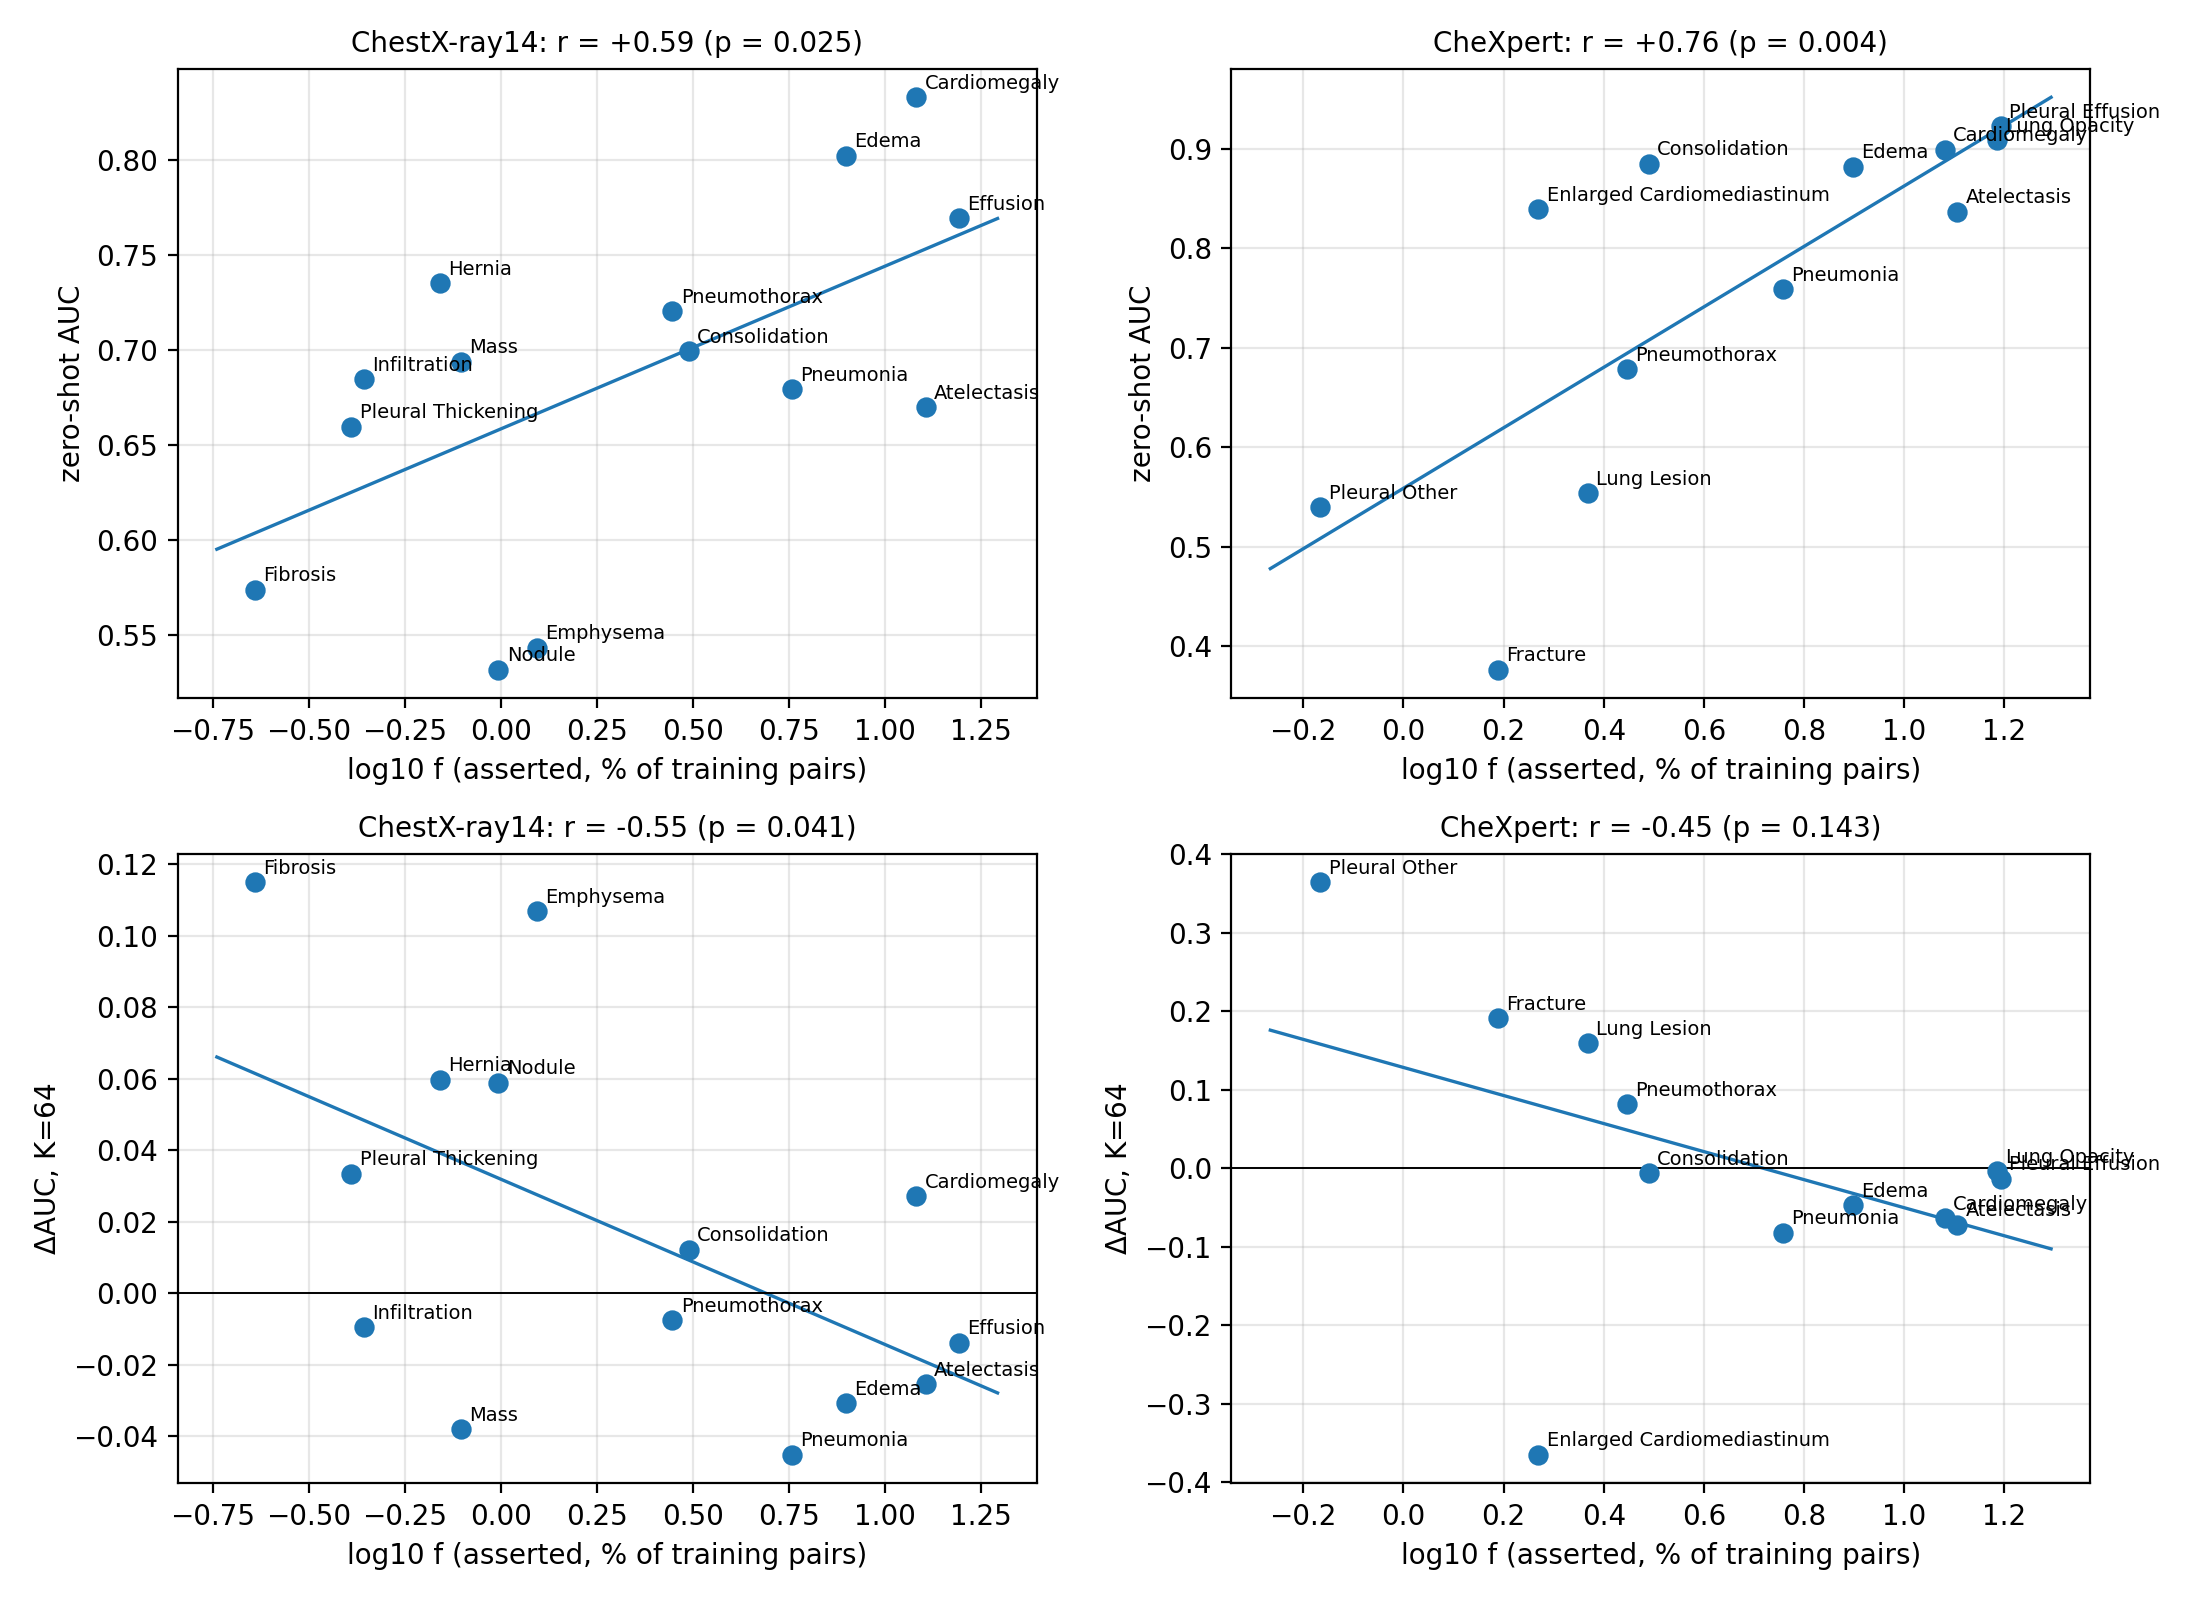
\includegraphics[width=0.85\textwidth]{figures/relationships.png}
\caption{Top: relationship (1), zero-shot AUC versus $\log_{10} f$ (asserted). Bottom: relationship (2),
few-shot gain $\Delta$AUC (SS-Text, $K=\KRef$) versus $\log_{10} f$. Left: ChestX-ray14; right: CheXpert.
Lines are least-squares fits.}
\label{fig:rel}
\end{figure*}

\subsection{Relationship (2): few-shot gain}
With SS-Text at $K=\KRef$, \NihImproved{} of 14 ChestX-ray14 classes and \CxpImproved{} of 12 CheXpert
classes improved over zero-shot. The gain decreased with log-frequency (Table~\ref{tab:rel}): $r=\NihRTwo$
($p=\NihPTwo$) on ChestX-ray14 and $r=\CxpRTwo$ ($p=\CxpPTwo$) on CheXpert. After controlling for
zero-shot AUC, the association was not significant on either test set (partial $r=\NihPartial$,
$p=\NihPartialP$; $r=\CxpPartial$, $p=\CxpPartialP$). Rarely asserted classes tended to have a lower
zero-shot AUC (relationship 1), and a lower zero-shot AUC went with a larger gain (ChestX-ray14
$r=\NihZsGainR$, $p=\NihZsGainP$; CheXpert $r=\CxpZsGainR$, $p=\CxpZsGainP$), although the rank
correlations were not significant ($\rho=\NihZsGainRho$, $p=\NihZsGainPs$; $\rho=\CxpZsGainRho$,
$p=\CxpZsGainPs$).

The correlation of $\log_{10} f$ with AUC also fell as $K$ grew (descriptive; not formally tested): from \NihTrendZero{} at $K=0$ to \NihTrendRef{} at $K=\KRef$ on ChestX-ray14
(for $K=0,1,2,\ldots,64$: \NihTrendAll) and from \CxpTrendZero{} to \CxpTrendRef{} on CheXpert.

\subsection{Image weight}
\begin{table*}[!t]
\centering
\footnotesize
\caption{Few-shot adaptation with three image weights: mean AUC over classes (each class: mean of 20 draws of the
support images). SS-Text: $\alpha=1$ as in~\cite{silvarodriguez2025fca}. Global $\alpha$ and the frequency rule
were chosen on the ChestX-ray14 selection set and applied to CheXpert without retuning.}
\label{tab:weight}
\begin{tabular}{lrrrrrr}
\toprule
 & \multicolumn{3}{c}{ChestX-ray14 test (14 classes)} & \multicolumn{3}{c}{CheXpert test (12 classes)} \\
$K$ & SS-Text & global $\alpha$ & frequency rule & SS-Text & global $\alpha$ & frequency rule \\
\midrule
0 (zero-shot) & 0.685 & 0.685 & 0.685 & 0.757 & 0.757 & 0.757 \\
1 & 0.601 & 0.687 & 0.687 & 0.653 & 0.758 & 0.759 \\
2 & 0.622 & 0.688 & 0.689 & 0.666 & 0.762 & 0.766 \\
4 & 0.637 & 0.691 & 0.691 & 0.685 & 0.767 & 0.767 \\
8 & 0.664 & 0.698 & 0.700 & 0.712 & 0.777 & 0.783 \\
16 & 0.685 & 0.703 & 0.705 & 0.725 & 0.779 & 0.784 \\
32 & 0.699 & 0.709 & 0.712 & 0.756 & 0.800 & 0.806 \\
64 & 0.703 & 0.710 & 0.713 & 0.769 & 0.810 & 0.814 \\
\bottomrule
\end{tabular}
\end{table*}

With $\alpha=1$, SS-Text at $K=\KRef$ left \NihFcaBelow{} of 14 ChestX-ray14 classes and \CxpFcaBelow{}
of 12 CheXpert classes below their zero-shot AUC (Table~\ref{tab:weight}). The global $\alpha$ chosen on
the selection set was \AlphaGlobalRef{} at $K=\KRef$, and it was better than $\alpha=1$ at every $K$ on
both test sets. At $K=\KRef$ the paired difference in mean AUC was \NihGlobalVsFca{} on ChestX-ray14 and
\CxpGlobalVsFca{} on CheXpert (95\% intervals).

The frequency rule chose $b<0$ at \RuleBNeg{} of \NK{} values of $K$ ($b=\RuleB$ at $K=\KRef$, giving
$\alpha_c$ from \AlphaRuleMin{} for the most to \AlphaRuleMax{} for the least frequent ChestX-ray14
class). It added a small gain over the global $\alpha$: \NihRuleVsGlobal{} on ChestX-ray14 and
\CxpRuleVsGlobal{} on CheXpert at $K=\KRef$. Per class, the number of classes significantly worse than
zero-shot fell from \NihFcaSigWorse{} (SS-Text) to \NihGlobalSigWorse{} (global $\alpha$) and \NihRuleSigWorse{}
(frequency rule) on ChestX-ray14, and from \CxpFcaSigWorse{} to \CxpGlobalSigWorse{} and \CxpRuleSigWorse{} on CheXpert.

% =================================================================================================
\section{Discussion}

The claim that zero-shot performance is limited by pretraining frequency, and that this is why
adaptation is needed~\cite{silvarodriguez2025fca}, is half supported in this radiology model. Classes
asserted more often in the training reports had higher zero-shot AUC on both test sets, in line with the
log-linear trend reported for general-domain models~\cite{udandarao2024zeroshot}. Rarely asserted classes
also tended to gain more from few-shot adaptation, but we found no significant association between
frequency and the gain once the zero-shot AUC was controlled for, and the zero-shot AUC was itself
associated with the gain.

\emph{Adaptation can harm.} 
Averaged over classes, SS-Text with its published weighting improved on zero-shot at $K=\KRef$, but it lowered the AUC of many classes, mostly frequently asserted ones. 
Averages hide this. A smaller image weight keeps more of the prompt and reduced this harm; the weight chosen on ChestX-ray14 transferred to CheXpert.

Varying $\lambda$
in SS-Text is not new: \cite{silvarodriguez2025fca} compared fixed values with their adaptive choice,
averaged over nine datasets, with ConVIRT as the chest X-ray model. Our contribution here is the
per-class view in CheXzero, where a smaller weight than the published one was better on both test sets.

\emph{Frequency as a prior for adaptation.} Setting the image weight per class from $f$ gave a small
further gain on both test sets. Its value is that $f$ comes from the pretraining text: once the two
numbers of the rule are fixed, a new test set needs no labelled images to set its weights, as on
CheXpert, where several classes do not occur in ChestX-ray14. The gain is small, and most of the improvement over SS-Text comes from the smaller weight itself.

\emph{Robustness.} Following the multiverse and specification-curve
recommendations~\cite{steegen2016multiverse,simonsohn2020specification}, we report relationships (1)
and (2) under several frequency definitions on ChestX-ray14. Directions agreed; significance at the 0.05
level did not always, so the results should be read as indicative.

\subsection{Limitations}
(i) $n=14$ and $n=12$ classes and one model. (ii) The mention phrases for the 7 classes the CheXpert
labeler does not cover are our own and cannot be checked against released labels. (iii) The image weight
and the frequency rule were chosen with the labels of 6{,}000 ChestX-ray14 selection images; the
bootstrap intervals resample test images only and do not include the variability of the support draws.
(iv) Few-shot results depend on the SS-Text weighting; we follow the paper's Eq.~10 with
$\lambda=1/(N\tau)$, whereas the authors' released code uses $\lambda=1/N$, which weights the image
embeddings by $1/\tau$ instead of 1. (v) Several CheXpert
classes have very few test positives (Table~\ref{tab:cxpclasses}), so their AUCs are noisy. (vi) The
ChestX-ray14 selection and support sets are split by image, not by patient (neither overlaps the test
set). (vii) ChestX-ray14 labels were mined from reports~\cite{wang2017chestxray8} and are noisy.

% =================================================================================================
\section{Conclusion}
How often a finding is asserted in the pretraining reports was associated with the zero-shot AUC of a chest X-ray
vision--language model on two test sets, but not with the benefit of few-shot adaptation once the
zero-shot AUC was controlled for. With its published weighting, the few-shot method lowered the AUC of many
classes, mostly frequently asserted ones; a smaller image weight, optionally set per class from pretraining frequency,
reduced this harm.

\bibliographystyle{IEEEtran}
\bibliography{references}

\end{document}
